\chapter{Verifica e Validazione}
\label{cap:verifica-validazione}
\section{Scopo del capitolo}
Questo capitolo descrive come è stata attuata la verifica e la validazione all'interno del progetto. Grazie al processo di verifica garantiamo che ogni attività dei processi svolti non introduca errori nel prodotto e che soddisfi i requisiti. Mentre con il processo di validazione viene determinato in maniera oggettiva che il prodotto sia conforme ai requisiti richiesti.
\section{Processo di verifica}
Durante tutto il periodo di tirocinio, ad ogni avanzamento di funzionalità e quindi cambio di requisito da soddisfare, con il tutor Antonio Fasolato è stato verificato che il codice sviluppato fino a quel momento fosse conforme con quanto aspettato e producesse output veritieri. Questo era aiutato inoltre dai controlli di validazione effettuati nei vari Controller e ulteriori controlli inseriti nei Service per garantire l’utilizzo di valori corretti.\\
Svolgendo le seguenti analisi regolarmente è stato possibile identificare e correggere errori evitando la loro propagazione nel corso della Codifica.
\subsection{Analisi statica}
Veniva effettuata un’analisi statica, che non richiede l'esecuzione del software, sul codice prodotto, eseguendo prima un inspection, una lettura mirata e focalizzata sugli errori più noti e probabili, andando verso errori più specifici in base alla funzionalità implementata.
\subsection{Analisi dinamica}
L'analisi dinamica consiste nell'effettuare test sul prodotto in esecuzione ed è stata eseguita nei seguenti modi.\\
Per identificare al meglio un errore a run-time veniva usata la tecnica di debugging: consiste nell'individuazione e la correzione di errori che provocano anomalie rilevate durante l'esecuzione del programma. Questa tecnica è possibile grazie allo strumento di debugging che offre IntelliJ che permette di inserire dei breakpoint, cioè dei punti di interruzione nel codice, che non appena raggiunti durante l'esecuzione, sospende l'esecuzione ed è possibile ispezionare lo stato delle variabili, delle strutture dati e lo stack trace delle chiamate.\\ 
Per testare l'API veniva utilizzato il software Postman. Esso permetteva di osservare la response dell'endpoint in analisi per verificare che fosse conforme alle attese e in caso di errore veniva eseguita un’ulteriore verifica successivamente alla mia correzione dell’errore che si era presentato.\\

\section{Testing}
Per garantire la sicurezza e l’affidabilità, negli ultimi giorni di tirocinio, sono stati introdotti i test di unità.\\
Questo processo è iniziato con lo studio dei framework JUnit e Mockito.\\
I test di unità verificano il funzionamento corretto di singole unità di codice, come metodi o classi. Questi test vengono sviluppati isolandosi dalle dipendenze esterne permettendo di verificare che il codice funzioni correttamente e che produca risultati attesi.\\
È stato ritenuto ragionevole testare ciò che io avevo prodotto come metodi o classi. Componenti introdotti da librerie o framework non hanno necessitato di test, dando per assodato il loro funzionamento.\\
Dato il poco tempo rimanente, per mettere in pratica quanto appreso, si è deciso di limitare lo svolgimento dei test su un \textit{@Service} semplice, \texttt{MilestoneService}, andando a testare il corretto funzionamento dei suoi metodi.

\subsection{Esempio di un test effettuato}
\begin{figure}[H] 
    \centering 
    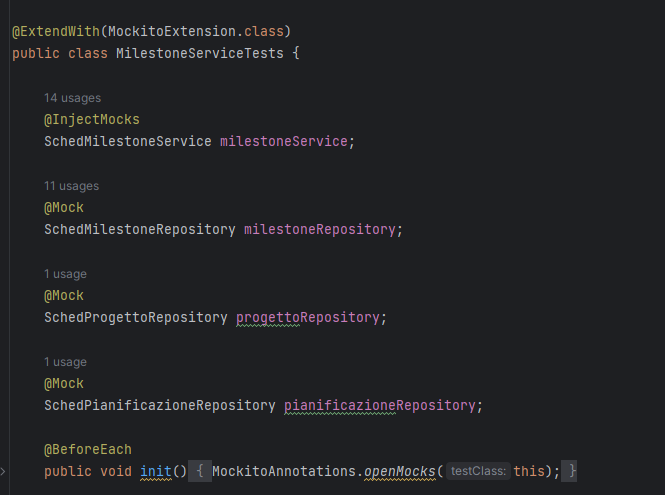
\includegraphics[width=0.85\columnwidth]{config-test} 
    \caption{Configurazione ambiente di testing}
\end{figure}
Per poter eseguire dei test su oggetti simulati (mock) , sono stati utilizzate le seguenti componenti.\\
Tramite l'annotazione \textit{@Mock} sono stati creati i componenti mock da iniettare all’interno del Service sotto test tramite l’annotazione \textit{@InjectMocks}. Tramite il metodo \texttt{init()}, annotato con \textit{@BeforeEach}, inizializziamo i metodi che vogliamo mockare permettendo l’utilizzo delle annotazioni che Mockito fornisce.\\
Qui riporto un code snippet dei controlli eseguiti nel test relativo al metodo di creazione di una nuova Milestone. Per garantire il corretto funzionamento della creazione della Milestone, è stata testata ogni parte delicata che avrebbe compromesso il funzionamento del metodo ,controllando l’eccezione sollevata, al momento dell’errore, assicurando che fosse quella corretta.\\

\begin{figure}[H] 
    \centering 
    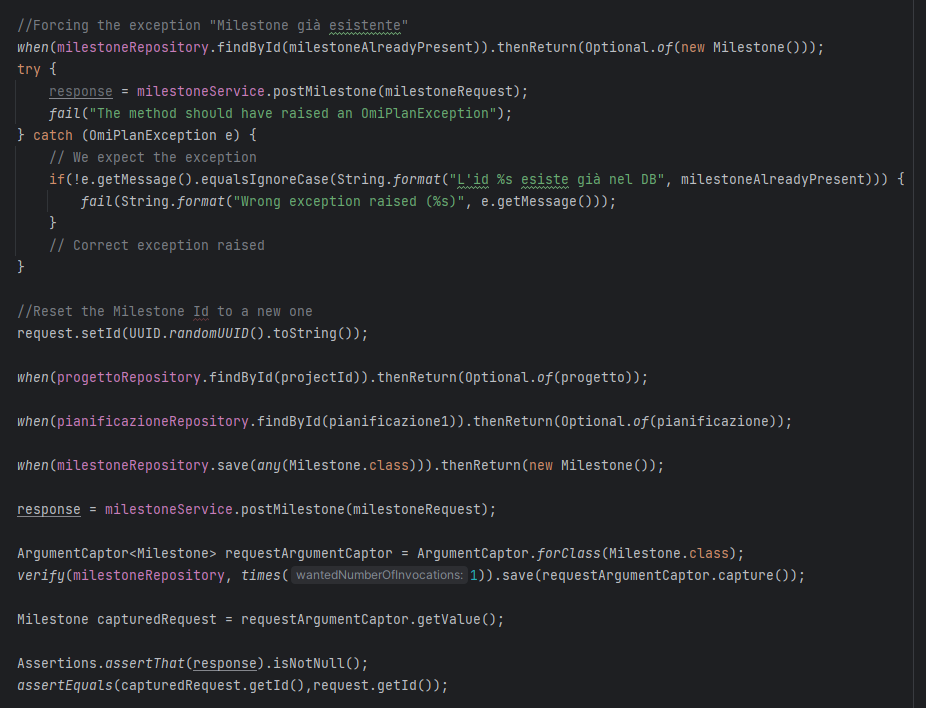
\includegraphics[width=0.9\columnwidth]{snippet-saveMilestone} 
    \caption{Code snippet test di creazione di una nuova Milestone}
\end{figure}

\noindent In questo snippet possiamo osservare come è stata forzata il lancio dell’eccezione quando si va a creare una Milestone con Id già esistente, controllando che sia stata proprio quella l’eccezione lanciata dal metodo.\\
Mockito offre strumenti, come il metodo \texttt{when()}, che consentono di effettuare stubbing\textsubscript{g} dei metodi, simulando il loro comportamento. Questo permette di definire come tali metodi dovrebbero rispondere quando vengono invocati, restituendo risultati specifici anziché eseguire il codice reale.\\ 
Un ulteriore metodo fornito da Mockito è \texttt{verify()}, utilizzato per controllare che il metodo \texttt{save()} della repository della Milestone venga chiamato una sola volta. Con \texttt{ArgumentCaptor<>} (che permette di raccogliere i parametri passati in una funzione) andiamo a "catturare" la Milestone salvata col metodo \texttt{save()}.\\
Per accertare che questa parte di test abbia avuto successo è stato verificato che la response ricevuta dal metodo non sia vuota e, dato che il DTO restituito differisce per alcune caratteristiche dall’istanza completa di una Milestone, non è stato possibile un confronto intero tra i due oggetti, ed è stato ritenuto esaustivo garantire l’uguaglianza dei due Id. Queste verifiche sono state effettuate tramite metodi di asserzione forniti da JUnit.
Con l’ausilio di questi metodi è stato possibile simulare la corretta creazione di una Milestone.\\

\section{Validazione}
Nell’ultimo giorno di tirocinio si è tenuto un incontro conclusivo insieme al tutor Antonio Fasolato e al \textit{RUOLO\_LAVORATIVO} Giovanni Incammicia, a conferma definitiva della conformità alle specifiche richieste del prodotto finale. Durante questa riunione, è stata effettuata una revisione dell'Analisi dei Requisiti fornita all'inizio del progetto, con particolare attenzione ai requisiti di mia competenza, al fine di verificare il loro soddisfacimento. Tuttavia, per scrivere il codice dell’API, è stato utilizzato principalmente un disegno iniziale dell’API e l’Analisi dei Requisiti fornita è stata utilizzata per aiutare la comprensione di alcuni endpoint. Questo approccio ha comportato alcune discrepanze tra le funzionalità implementate e i requisiti specificati. Rispetto all’Analisi dei Requisiti mancavano degli attributi che il Front-end necessitava o alcune funzionalità che necessitavano implementazioni particolari o di collegamenti a servizi esterni di cui non c’era tempo a sufficienza per poter studiare. Nonostante queste mancanze, analizzando le funzionalità implementate e le response fornite, è stato ritenuto sufficiente per il soddisfacimento dei requisiti di cui gli endpoint sviluppati facevano parte.\\
A causa delle problematiche da me sopra menzionate, non è stato possibile condurre una fase di Collaudo effettiva per valutare l'interazione tra il Front-end e il Back-end.